\documentclass[aspectratio=169, 10pt, handout,usenames,dvipsnames]{beamer}

\usecolortheme{dove}
\definecolor{mycyan}{rgb}{0.2157, 0.7059, 0.9608}
\setbeamercolor{alerted text}{fg=mycyan}
\setbeamertemplate{bibliography item}{\insertbiblabel}
\setbeamertemplate{caption}[numbered]
\hypersetup{colorlinks,linkcolor=,urlcolor=mycyan}
\usepackage{animate,xcolor,colortbl,listings,nicefrac}
\usepackage[italian]{babel}
\usepackage{verbatim}
\usepackage{mathtools}
\setbeamertemplate{footline}[frame number]
\usepackage{listings}
\lstset{upquote=false}
\usepackage[]{framed}
\usepackage{xfrac}
\usepackage{multicol}
\usepackage{cellspace}
\usepackage{tikz}
\usepackage[american,nooldvoltagedirection,europeanvoltages]{circuitikz}
\setlength\cellspacetoplimit{4pt}
\setlength\cellspacebottomlimit{4pt}
\setbeamercolor{alerted text}{fg=Cerulean}

\newcommand{\circuito}{
    \draw (0,0)
        to[american voltage source,invert, l=$V_{in}(t)$] (0,3)
        -- (0.5,3)
        to[L=$L$] (2,3)
        to[R=$R1$] (5,3)
        to[R=$R2$] (5,0)
        -- (0,0);
    \draw (5,3)
        -- (7,3)
        to[C, l=$C$] (7,0) -- (5,0);
    \draw
        (7,3) to[short, -o]
        node[anchor=west]{} (8,3);
    \draw
        (7,0) to[short, -o]
        node[anchor=west]{} (8,0);
    \draw
     (8,3) to[open, v^<=$V_{out}$] (8,0);
    }

\title{Metodi multistep: BDF e sistemi stiff}

\date{27/05/2020}
\author{Giacomo Tombolan \and Valerio Nappi \and
      Lorenzo Rossi \and  \texorpdfstring{\\ }  MMarco Manganini \and
      Mirko Seghezzi}

\begin{document}

\begin{frame}
  \maketitle
\end{frame}


\begin{frame}


  \frametitle{Bibliografia}
  \begin{thebibliography}{99}\small

    \bibitem{quarteroni2012calcolo}
    Quarteroni A., Saleri F. and Gervasio P.
    \newblock {\em Calcolo Scientifico: Esercizi e problemi risolti con MATLAB e  Octave}.
    \newblock UNITEXT. Springer Milan, 2012.

    \bibitem{petzold}
    Ascher Uri M. and Petzold Linda R.
    \newblock {\em Computer methods for ordinary differential equations and differential-algebraic equations}.
    \newblock Siam, 1998.

    \bibitem{robertson}
    Robertson H. H. "The Solution of a Set of Reaction Rate Equations"
    \newblock {in: Walsh J. (ed.), \em Numerical Analysis. An Introduction based on a Symposium Organized by the Institute of Mathematics and its Applications}.
    \newblock Academic Press, 1972. pp 178-182
    \bibitem{BDF_Scholarpedia}
    Gear B.
    \newblock Backward Differentiation Formulas (Scholarpedia)
    \newblock \url{http://www.scholarpedia.org/article/Backward_differentiation_formulas}
<<<<<<< HEAD

=======

>>>>>>> 12a297c... aggiornate slides, rimosso submodule

   \end{thebibliography}

%Una volta inserito un documento in bibliografia,
%può essere citato così:~\cite{quarteroni2012calcolo}

\end{frame}




\begin{frame}
  \frametitle{Sommario}
  %Questo comando inserisce una lista delle sezioni in
  %cui è divisa la presentazione. Perché una sezione appaia
  %nel sommario deve contenere almeno una pagina.
  \tableofcontents
\end{frame}


\section{Introduzione a sistemi stiff e metodi BDF}\label{sec:sec1}
\begin{frame} \frametitle{Introduzione a sistemi stiff e metodi BDF}
    \begin{itemize}
        \item I sistemi stiff sono problemi molto comuni nel campo dell'elettronica.
        \item Analizzeremo dei metodi per risolverli efficacemente
        \item Ma prima di dare definizioni...
    \end{itemize}
\end{frame}


\section{Analisi del circuito RLC}\label{sec:sec2}

\begin{frame}{Circuito RLC}
Si supponga di prendere in esame il seguente circuito, con l'obiettivo di calcolarne la tensione di uscita \( V_{out} \) considerando uno scalino ritardato in ingresso, di ampiezza \( V_{in} \)

            \begin{center}
                    \begin{circuitikz}[scale=1]
                \circuito
                \end{circuitikz}
            \end{center}

\end{frame}

\begin{frame}{Analisi del circuito RLC}
Analizziamo il circuito attraverso la legge di Kirchhoff delle correnti e quella delle tensioni. Prendiamo in considerazione la maglia \textcolor{Cerulean}{azzurra} e il nodo \textcolor{BurntOrange}{arancione}.
\vspace{0.3cm}
    \begin{multicols}{2}
    \begin{center}
    \hspace*{-0.5cm}
        \begin{circuitikz}[scale=0.8]
        \circuito
        \draw [Cerulean, thick, latex-] (2.5,0.5) arc (-90:175:10mm) ;
        \draw [Cerulean] (2.5,1.5)node{KLV};
        \draw [BurntOrange, thick] (4.5,3.6) rectangle (7.5,2.6);
        \draw [BurntOrange] (6,3) node[above] {KLC};
        \end{circuitikz}

    \end{center}

    \columnbreak

    \hspace*{1.7cm}\begin{minipage}{\textwidth}
        \large
        $\begin{cases}
           \textcolor{Cerulean}{KLV:}  V_{in} = V_L + V_{R1} + V_{out} \\
<<<<<<< HEAD
           \textcolor{BurntOrange}{KLC:}  I_{in} =  I_{R2} + I_C
=======
           \textcolor{BurntOrange}{KLC:}  I_{in} =  I_{R2} + I_C
>>>>>>> 12a297c... aggiornate slides, rimosso submodule
        \end{cases} $
        \medskip\\
        $\begin{cases}
            {x_1} = V_{out}\\
<<<<<<< HEAD
            {x_2} = I_{in}
=======
            {x_2} = I_{in}
>>>>>>> 12a297c... aggiornate slides, rimosso submodule
        \end{cases} $
        \bigskip\\
        Otteniamo il sistema:\medskip\\
        $\begin{cases}
            \dot{x_1} = -\dfrac{1}{L}x_1 - \dfrac{R_1}{L}x_2 + \dfrac{1}{L}V_{in}\\
<<<<<<< HEAD
            \dot{x_2} = -\dfrac{1}{R_2 C}x_1 + \dfrac{1}{C}x_2
=======
            \dot{x_2} = -\dfrac{1}{R_2 C}x_1 + \dfrac{1}{C}x_2
>>>>>>> 12a297c... aggiornate slides, rimosso submodule
        \end{cases}$
        \end{minipage}
    \end{multicols}
\end{frame}

\begin{frame}{Analisi del circuito RLC: rappresentazione matriciale}
Possiamo riscrivere il sistema ottenuto come matrice:

%\renewcommand\arraystretch{2.3} % vengono circa alte uguali ma il testo non è centrato
\large
\begin{center}
\[
<<<<<<< HEAD
    \begin{bmatrix}
    \dot{x_1} \\
    \dot{x_2} \end{bmatrix}  =
    \begin{bmatrix}
    -\dfrac{1}{L} & - \dfrac{R_1}{L}\\[1.5ex]
    -\dfrac{1}{R_2C} & + \dfrac{1}{C}
    \end{bmatrix}
    \begin{bmatrix}
    x_1 \\
    x_2 \end{bmatrix}
    +
    \begin{bmatrix}
    0 \\[1.5ex]
    -\dfrac{1}{L}
    \end{bmatrix}
    \begin{bmatrix}
    0 \\
    V_{in}
=======
    \begin{bmatrix}
    \dot{x_1} \\
    \dot{x_2} \end{bmatrix}  =
    \begin{bmatrix}
    -\dfrac{1}{L} & - \dfrac{R_1}{L}\\[1.5ex]
    -\dfrac{1}{R_2C} & + \dfrac{1}{C}
    \end{bmatrix}
    \begin{bmatrix}
    x_1 \\
    x_2 \end{bmatrix}
    +
    \begin{bmatrix}
    0 \\[1.5ex]
    -\dfrac{1}{L}
    \end{bmatrix}
    \begin{bmatrix}
    0 \\
    V_{in}
>>>>>>> 12a297c... aggiornate slides, rimosso submodule
    \end{bmatrix}
\]
\end{center}
\normalsize
Prendiamo in considerazione la matrice dei coefficienti del sistema:
\large\medskip
\[ A = \begin{bmatrix}
-\dfrac{1}{L} & - \dfrac{R_1}{L}\\[1.5ex]
-\dfrac{1}{R_2C} & + \dfrac{1}{C}
\end{bmatrix} \]

\end{frame}

\begin{frame}{Analisi del circuito RLC: gli autovalori}
    \begin{itemize}
        \item Dagli autovalori di questa matrice discendono importanti proprietà del sistema:
        \medskip
        \[
        eig(A) \Rightarrow  \begin{vmatrix} -\dfrac{1}{L}-\lambda & - \dfrac{R_1}{L}\\[1.5ex] -\dfrac{1}{R_2 C} & + \dfrac{1}{C}-\lambda \end{vmatrix} = 0
        \]
        \medskip
        \[
        \lambda_{1,2}  = -\frac{L \pm \sqrt{(C R_1 R_2 - L)^2 - 4CL R_2 ^2} + C R_1 R_2} {2 C L R_2}
        \]
        \medskip
        \item La soluzione libera del sistema sarà una combinazione lineare dei \alert{modi} del sistema: \( e^{\lambda_nt}\)
        \item Per $\lambda$ positivi il sistema diverge per $t \rightarrow \infty $. Chiediamo quindi autovalori con $\operatorname{\mathbb{R}e}(\lambda)<0$
<<<<<<< HEAD
        \item La soluzione è dominata dall'autovalore \alert{più piccolo}, che individua il polo dominante.
=======
        \item La soluzione è dominata dall'autovalore \alert{più piccolo}, che individua il polo dominante.
>>>>>>> 12a297c... aggiornate slides, rimosso submodule
        \item Numericamente non possiamo permetterci di trascurare gli altri autovalori.


 \end{itemize}
\end{frame}



    \begin{frame}{Assoluta stabilità}
        Dagli autovalori dipende inoltre la stabilità della risoluzione numerica.\\
        Come visto a lezione, con il metodo di Eulero esplicito abbiamo assoluta stabilità se \(|1+h\lambda| < 1\), con $h$ passo di discretizzazione della variabile indipendente\\
        Dovremo quindi scegliere un passo $h$ tale che la relazone sia soddisfatta per \alert{tutti} gli autovalori
        \medskip
        \begin{multicols}{2}
        \begin{figure}
        \centering
        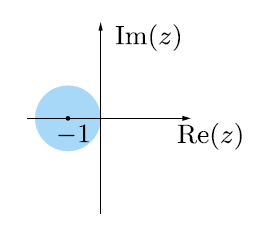
\includegraphics[width=0.8\linewidth]{fig6.png}
        \label{fig:festability}
        \end{figure}
        \columnbreak
        \bigskip\bigskip
        Osserviamo poi che per autovalori reali, la relazione si riduce a: \large
        \[
        -2 < h \lambda_n < 0 \qquad \forall n
        \] \normalsize
        O in modulo, assunto $\lambda<0$: \large
        \[
        |h \lambda_n| < 2 \qquad \forall n
        \]
        \end{multicols}

    \end{frame}
<<<<<<< HEAD

=======

>>>>>>> 12a297c... aggiornate slides, rimosso submodule
\section{Cosa sono i sistemi Stiff?}\label{sec:sec3}
\begin{frame} \frametitle{Cosa sono i sistemi Stiff?}
    \begin{itemize}
        \item Sono sistemi caratterizzati da modi (autovalori) distanti di molti ordini di grandezza tra di loro.
        \item Più è grande la differenza tra la componente più lenta e la più veloce, più il sistema è stiff.
        \item La stiffness è una proprietà associata al sistema sotto analisi
    \end{itemize}
\end{frame}

\begin{frame}{Esempio: circuito RLC \alert{non} stiff}
Si supponga di prendere in esame il seguente circuito, con l'obiettivo di calcolarne la tensione di uscita \( V_{out}(t) \) considerando un generatore di tensione forzante \( V_{in} \)
        \begin{multicols}{2}
        \begin{center}
        \begin{circuitikz}[scale=0.8]
        \circuito
        \end{circuitikz}
        \end{center}

          \begin{figure}
       \centering 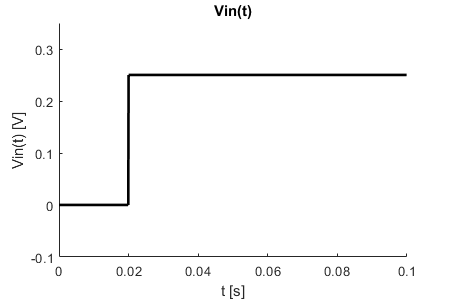
\includegraphics[width=0.6\linewidth]{vin.png}
        \label{fig:vin_nonstiff}
        \end{figure}

    \columnbreak
    \bigskip
    \bigskip
    \hspace{2.5cm}
        $\begin{cases}
            L = 67 \; m H \\
            C = 760 \; \mu F \\
            R_1 = 20 \; \Omega \\
            R_2 = 1 \; k\Omega\\
            %V_{in} = V_0 \cdot \sin(2 \pi \omega t) \; V
            V_{in} = \; Vu(t-0.02)
        \end{cases}$ \\
        \bigskip
        \bigskip
    \hspace{2.5cm}
    \fcolorbox{blue}{white}{
        $\begin{cases}
        \lambda_1 = -100\\
        \lambda_2 = -200 \;
        \end{cases}$}
    \end{multicols}
\end{frame}

\begin{frame}{Esempio: circuito RLC \alert{non} stiff - soluzione}
Il valore di \( V_{out}(t) \) è facilmente calcolato usando, ad esempio, un metodo esplicito (Eulero in avanti).\\ \medskip
È necessario scegliere un passo di discretizzazione $h$ che soddisfi la relazione $|h \lambda_n| < 2$\\     \bigskip
    \begin{multicols}{2}
        \begin{figure}
       \centering        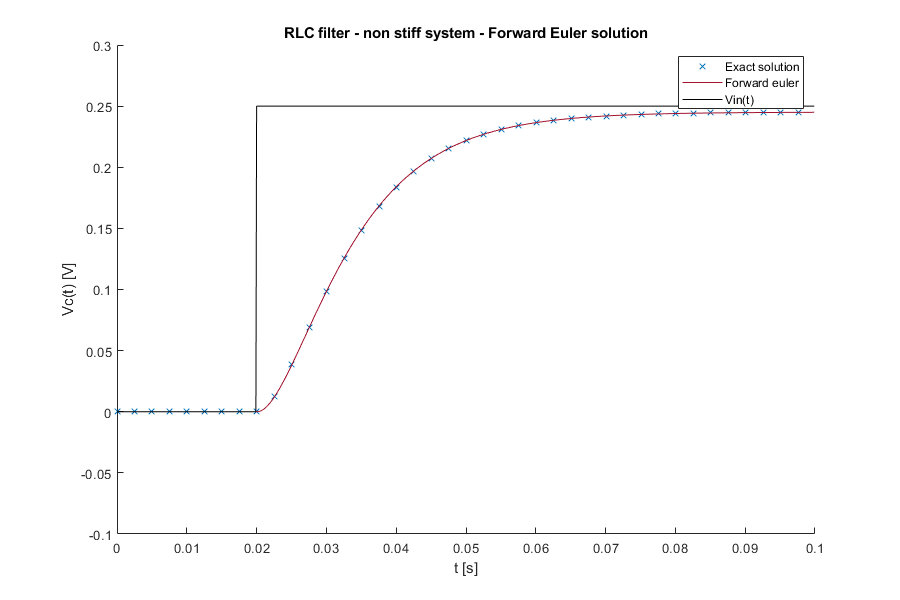
\includegraphics[width=1.05\linewidth]{rlc_non_stiff_forward_euler.png}
        \label{fig:fe_nonstiff}
        \end{figure}
    \columnbreak
    \begin{itemize}
    \item Dobbiamo soddisfare la condizione più stringente: $|h \lambda_2| < 2$
    \[
    h < \dfrac{1}{100}
    \]
    \item Valutando il sistema per $t\in [0,0.1]$ dovremo eseguire \alert{più di 10 passi}.
    \item La condizione è facilmente soddisfatta, scegliamo infatti di eseguire 100 passi per avere un numero apprezzabile di punti.
    \end{itemize}
    \end{multicols}

\end{frame}

\begin{frame}{Esempio: circuito RLC stiff}
    Cambiando il valore dei componenti, il sistema dà origine ad autovalori differenti tra di loro di parecchi ordini di grandezza
        \begin{multicols}{2}
            \begin{center}
                \begin{circuitikz}[scale=0.8]
                \circuito
                \end{circuitikz}
            \end{center}

                          \begin{figure}
       \centering 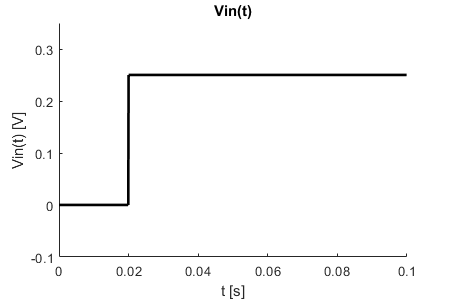
\includegraphics[width=0.6\linewidth]{vin.png}
        \label{fig:vin_stiff}
        \end{figure}
    \columnbreak
    \hspace{2.5cm}
    \medskip
        $\begin{cases}
            L = 20 \; \mu H \\
            C = 500 \; \mu F \\
            R_1 = 20 \; \Omega \\
            R_2 = 1 \; k\Omega\\
            V_{in} = \; Vu(t-0.02)
        \end{cases}$ \\
        \bigskip
        \bigskip
    \hspace{2.5cm}
    \fcolorbox{red}{white}{
        $\begin{cases}
            \lambda_1 = -100\\
            \lambda_2 = -1000000 \;
        \end{cases}$}
    \end{multicols}
\end{frame}

\begin{frame}{Circuito RLC con eulero in avanti}
Se volessimo risolvere il nuovo sistema \alert{stiff}, dovremmo considerare un passo h molto più piccolo
\begin{multicols}{2}
        \begin{figure}
        \centering
        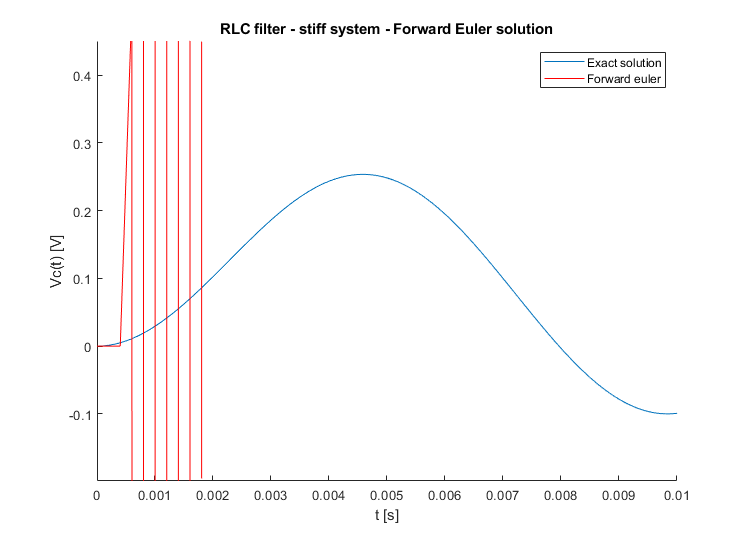
\includegraphics[width=1\linewidth]{rlc_forward_euler.png}
        \label{fig:fe_stiff}
        \end{figure}
        \begin{centering}
            Considerando lo stesso h utilizzato prima, considerando solo l'autovalore dominante, la soluzione diverge molto velocemente
        \end{centering}
        \columnbreak
        \begin{itemize}
    \item Dovremo soddisfare la relazione \( | h \lambda_2 < 2 | \) \[h < \dfrac{1}{500000} \]
    \item Questa scelta di h implicherebbe una esecuzione di oltre \alert{50000} passi
    \item Con 100000 passi, il tempo di simulazione da noi registrato è pari a circa 2.5 secondi

\item Ci servono nuovi metodi: BDF

\end{itemize}
\end{multicols}

\end{frame}



\begin{comment}
    \section{Problema risoluzione sistemi Stiff con metodi espliciti}\label{sec:sec4}

    \begin{frame}{Problema risoluzione sistemi Stiff con metodi espliciti}
        \begin{itemize}
            \item \alert{Problema modello}: con Eulero esplicito bisogna mirare al cerchio di raggio 1 (stabilità condizionata per semipiano negativo).
            \item Per autovalori enormi, se $h\lambda$ deve centrare il cerchio, allora h (passo di discretizzazione) deve essere estremamente piccolo
            \item Per autovalori infiniti (DAE) allora  $h\approx 0$  $\rightarrow$ impossibile
            \item Possiamo risparmiare calcoli mantenendo accuratezza? Possiamo aspirare a risolvere un sistema con DAE? Bisogna ricorrere a metodi impliciti
        \end{itemize}

        \begin{figure}
        \centering
        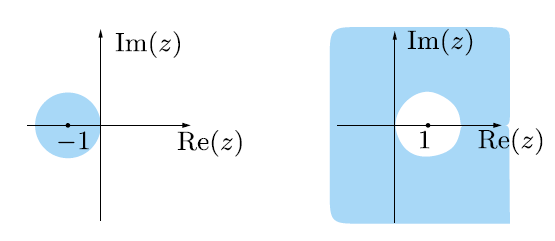
\includegraphics[width=.45\linewidth]{fig1.png}
        \caption{Per i metodi impliciti il semipiano reale negativo è tutto disponibile:\\
            \begin{itemize}
                \item h può variare incondizionatamente
                \item si possono risolvere problemi ad autovalori infiniti (DAE)
            \end{itemize}
        }
        \label{fig:my_label}
        \end{figure}
    \end{frame}
\end{comment}

\section{BDF}\label{sec:sec5}

    \begin{frame}{Backward Differentiation Formulas (BDF)}
        \begin{itemize}
            %\item Backward Differentiation Formulae: la valutazione n-esima dipende dalla storia passata delle valutazioni e dalla valutazione della f a passo n-esimo
            \item \textbf{Linear Multistep Methods (LMM)}: la valutazione n-esima dipende dalla storia passata delle valutazioni e dalla valutazione della f a passo n-esimo.
            %\item Anche se lineari risolvono comunque problemi non lineari
            \end{itemize}
            \textbf{Vantaggi:}
        \begin{itemize}
            %\item Richiedono meno valutazioni della funzione per ogni step (rispetto a Runge-Kutta)
            \item Migliore accuratezza rispetto ad altri metodi (es. RK) a parità di numero di valutazioni della funzione
<<<<<<< HEAD
            \item Metodi costruiti più semplici e performanti in fatto di ordine e stima dell’errore
=======
            \item Metodi costruiti più semplici e performanti in fatto di ordine e stima dell’errore
>>>>>>> 12a297c... aggiornate slides, rimosso submodule
            \item Proprietà di stiff decay
            %\item Migliore accuratezza rispetto a metodi one-step a parità di numero di valutazioni della funzione
        \end{itemize}
        \textbf{Svantaggi:}
        \begin{itemize}
            \item Necessità di condizioni iniziali accurate: alto costo computazionale di partenza
            \item Flessibilità minore per avere adattività di ordine e di passo di integrazione
            \item Per metodi multistep: zero stabilità da determinare (gli one step hanno la zero stabilità garantita dalla consistenza)
        \end{itemize}
            %\[ f(y_n, t_n) = \dfrac{1}{\beta_0}\dfrac{\sum_{j=0}^{k}\alpha_j y_{n-j}}{h } \]

            %\[ f(y_n, t_n) = \dfrac{1}{\beta_0}\dfrac{\sum_{j=0}^{k}\alpha_j y_{n-j}}{h } = \dfrac{1}{\beta_0}\dfrac{\alpha_0 y_n +\alpha_1 y_n-1 + ...}{h}\]


            %\[ f(y_n, t_n) = \dfrac{y_n}{h \beta_0} + \dfrac{1}{h \beta_0} \sum_{j=1}^{k}\alpha_j y_{n-j}\]

            %h\displaystyle\sum_{j=0}^k \beta_j f_{n-j} \]
    \end{frame}

    \begin{frame}{Costruiamo BDF}
        Dato il problema di Cauchy $y'=f(t,y)$
        \begin{itemize}
            \item costruiamo l'interpolante $\varphi(t)$ della soluzione $y$
            \[ y(t) \approx\varphi(t)= y(t_n) + (t-t_n)\dfrac{y(t_n)-y(t_{n-1})}{t_n-t_{n-1}}\]
            \item la deriviamo e la poniamo uguale a $f(t,y)$
            \[ y'(t)\approx \varphi'(t)=\dfrac{y(t_n)-y(t_{n-1})}{t_n-t_{n-1}}=\dfrac{y(t_n)-y(t_{n-1})}{h}=f(t_n,y_n)\]
            \item Più in generale, per ordini superiori al primo, possiamo scrivere: \\
            \begin{center}
            \begin{tabular}{c  c}
            \( f(t_n,y_n) = \dfrac{1}{\beta_0}\dfrac{\sum_{j=0}^{k}\alpha_j y_{n-j}}{h } \) &\space\space
            \( \displaystyle\sum_{j=0}^k \alpha_j y_{n-j} = h\beta_0 f(t_n,y_n) \)
            \end{tabular}
            \end{center}
            \item Espandiamo ora coefficienti ed equazioni

        \end{itemize}

    \end{frame}
\begin{comment}
    \begin{frame}{BDF (I)}
        \begin{itemize}
            \item Più in generale, per ordini superiori al primo, possiamo scrivere: \\
            \[ y_n=-\displaystyle\sum_{j=1}^k \alpha_j y_{n-j} + h\beta_0 f(t_n,y_n) \]

            \item Espandiamo ora coefficienti ed equazioni
        \end{itemize}
    \end{frame}
\end{comment}



\begin{comment}
    \begin{frame}{BDF (II)}
        \begin{itemize}
            \item \textbf{Caso più semplice di BDF :} Eulero implicito (BDF1)
            %\item Sono impliciti, non possiamo sfuggire dalla risoluzione di equazioni non lineari: necessitano di accoppiamento con metodi (es. Newton modificato) nell’implementazione.
        \end{itemize}

        %\begin{figure}
        %\centering
       % 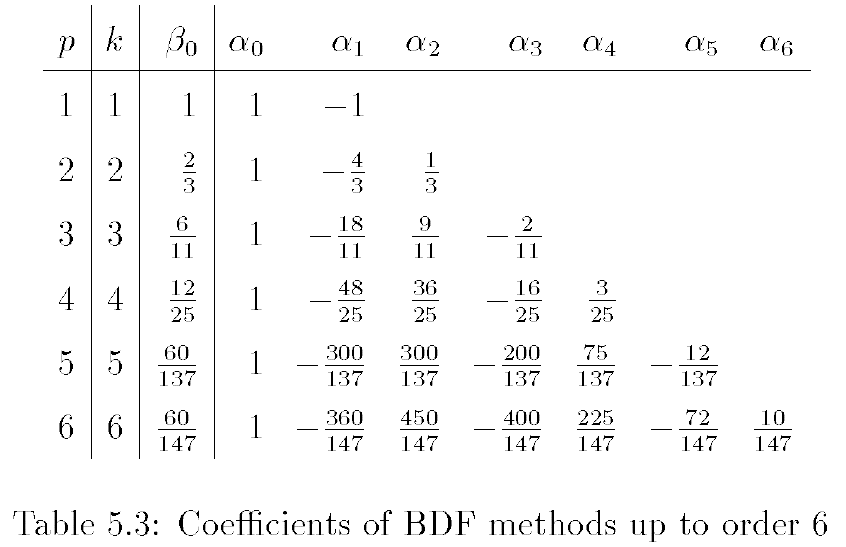
\includegraphics[width=.5\linewidth]{fig2.png}
        %\label{fig:my_label}
        %\end{figure}
        \begin{table}[]
            \begin{tabular}{Sc|Sc|Sc|ScScScScScScSc}
            \( p \) & \(k\) & \(\beta_0\) & \(\alpha_0\) & \(\alpha_1\) & \(\alpha_2\)  & \(\alpha_3\) & \(\alpha_4\) & \(\alpha_5\) & \(\alpha_6\) \\
            \hline
            \(1\) & \(1\) & \(1 \)       & \(1 \) & \(-1\)       &                             &          &         &         &        \\
            \(2\) & \(2\) & \(\sfrac{2}{3} \)    & \(1\) & \(\sfrac{4}{3} \)     & \(\sfrac{1}{3} \)                         &          &         &         &        \\
            \(3\) & \(3\) & \(\sfrac{6}{11} \)   & \(1\) & \(\sfrac{-18}{11} \)   & \(\sfrac{9}{11} \)                       & \(\sfrac{-2}{11}\)    &         &         &        \\
            \(4\) & \(4\) & \(\sfrac{12}{25} \)  & \(1\) & \(\sfrac{-48}{25} \)   & \(\sfrac{36}{25} \)   & \(\sfrac{-16}{25}\)   & \(\sfrac{3}{25}\)   &         &        \\
            \(5\) & \(5\) & \(\sfrac{60}{137} \) & \(1\) & \(\sfrac{300}{137} \)  & \(\sfrac{300}{137}\) & \(\sfrac{-200}{137}\) & \(\sfrac{75}{137}\)  & \(\sfrac{-12}{137}\) &        \\
            \(6\) & \(6\) & \(\sfrac{60}{147} \) & \(1\) & \(\sfrac{-360}{147} \) & \(\sfrac{450}{147}\) & \(\sfrac{-400}{137}\) & \(\sfrac{225}{147}\) & \(\sfrac{72}{147}\) & \(\sfrac{10}{147}\)
            \end{tabular}
        \end{table}
        \item BDF7 è instabile
    \end{frame}
\end{comment}

    \begin{frame}{BDF (II)}
        \begin{itemize}
            \item \textbf{Caso più semplice di BDF :} Eulero implicito (BDF1)
            %\item Sono impliciti, non possiamo sfuggire dalla risoluzione di equazioni non lineari: necessitano di accoppiamento con metodi (es. Newton modificato) nell’implementazione.
        \end{itemize}

        %\begin{figure}
        %\centering
       % 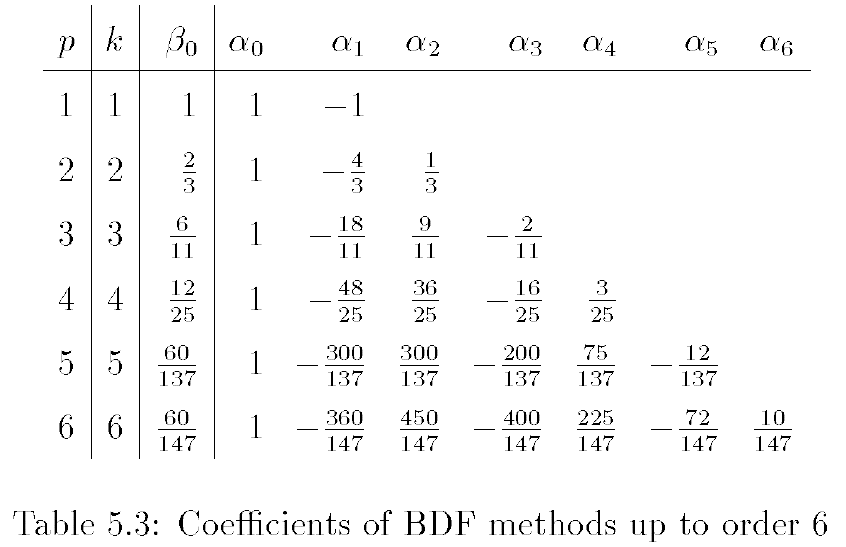
\includegraphics[width=.5\linewidth]{fig2.png}
        %\label{fig:my_label}
        %\end{figure}
        \begin{table}[]
            \begin{tabular}{Sc|Sc|Sc|ScScScScScScSc}
            \( BDF \)& \(\beta_0\) & \(\alpha_0\) & \(\alpha_1\) & \(\alpha_2\)  & \(\alpha_3\) & \(\alpha_4\) & \(\alpha_5\) & \(\alpha_6\) \\
            \hline
            \(BDF1\)& \(1 \)       & \(1 \) & \(-1\)       &                             &          &         &         &        \\
            \(BDF2\)& \(\sfrac{2}{3} \)    & \(1\) & \(\sfrac{4}{3} \)     & \(\sfrac{1}{3} \)                         &          &         &         &        \\
            \(BDF3\)& \(\sfrac{6}{11} \)   & \(1\) & \(\sfrac{-18}{11} \)   & \(\sfrac{9}{11} \)                       & \(\sfrac{-2}{11}\)    &         &         &        \\
            \(BDF4\)& \(\sfrac{12}{25} \)  & \(1\) & \(\sfrac{-48}{25} \)   & \(\sfrac{36}{25} \)   & \(\sfrac{-16}{25}\)   & \(\sfrac{3}{25}\)   &         &        \\
            \(BDF5\)& \(\sfrac{60}{137} \) & \(1\) & \(\sfrac{300}{137} \)  & \(\sfrac{300}{137}\) & \(\sfrac{-200}{137}\) & \(\sfrac{75}{137}\)  & \(\sfrac{-12}{137}\) &        \\
            \(BDF6\)& \(\sfrac{60}{147} \) & \(1\) & \(\sfrac{-360}{147} \) & \(\sfrac{450}{147}\) & \(\sfrac{-400}{147}\) & \(\sfrac{225}{147}\) & \(\sfrac{72}{147}\) & \(\sfrac{10}{147}\)
            \end{tabular}
        \end{table}
    \end{frame}



\begin{frame}{BDF (III)}
        \begin{itemize}
            \item {La tabella può essere meglio visualizzata scrivendo le equazioni $\alpha_j$ e $\beta_0$:}
        \end{itemize}

    \begin{center}
        \begin{table}[]
            \begin{tabular}{ScSl}
            BDF1 & \( y_n = y_{n-1} + h f(t_{n}, y_{n})\) \textcolor{red}{\( \rightarrow  y_{n} = -\alpha_1y_{n-1} + \beta_0h f(t_{n}, y_{n})\)}\\
            BDF2 & \(y_{n} = \tfrac43 y_{n-1} - \tfrac13 y_{n-2} + \tfrac23 h f(t_{n}, y_{n}) \) \textcolor{red}{\(\rightarrow y_{n} = -\alpha_1y_{n-1} -\alpha_2y_{n-2} + \beta_0h f(t_{n}, y_{n}) \)}\\
<<<<<<< HEAD

=======

>>>>>>> 12a297c... aggiornate slides, rimosso submodule
            BDF3 & ...\\%\(y_{n+3} = \tfrac{18}{11} y_{n+2} - \tfrac9{11} y_{n+1} + \tfrac2{11} y_n +\tfrac6{11} h f(t_{n+3}, y_{n+3}) \) \\
            BDF4 & ...\\ %\(y_{n+4} = \tfrac{48}{25} y_{n+3} - \tfrac{36}{25} y_{n+2} + \tfrac{16}{25} y_{n+1} - \tfrac{3}{25} y_n + \tfrac{12}{25} h f(t_{n+4}, y_{n+4}) \) \\
            BDF5 & ...\\ %\( y_{n+5} = \tfrac{300}{137} y_{n+4} - \tfrac{300}{137} y_{n+3} + \tfrac{200}{137} y_{n+2} - \tfrac{75}{137} y_{n+1} + \tfrac{12}{137} y_n + \tfrac{60}{137} h f(t_{n+5}, y_{n+5}) \)  \\
            BDF6 & \(y_{n} = \tfrac{360}{147} y_{n-1} - \tfrac{450}{147} y_{n-2} + \tfrac{400}{147} y_{n-3} - \tfrac{225}{147} y_{n-4} + \tfrac{72}{147} y_{n-5} - \tfrac{10}{147} y_{n-6} + \tfrac{60}{147} h f(t_{n}, y_{n}) \)
            \end{tabular}
        \end{table}
    \end{center}
\end{frame}


\begin{comment}
\section{Vantaggi e svantaggi}\label{sec:sec6}

    \begin{frame}{Vantaggi e svantaggi}
        \textbf{Vantaggi:}
        \begin{itemize}
            %\item Richiedono meno valutazioni della funzione per ogni step (rispetto a Runge-Kutta)
            \item Migliore accuratezza rispetto ad altri metodi (es. RK) a parità di numero di valutazioni della funzione
            \item Metodi costruiti più semplici e performanti in fatto di ordine e stima dell’errore
            %\item Migliore accuratezza rispetto a metodi one-step a parità di numero di valutazioni della funzione
        \end{itemize}
        \textbf{Svantaggi:}
        \begin{itemize}
            \item Necessità di condizioni iniziali accurate: alto costo computazionale di partenza
            \item Flessibilità minore per avere adattività di ordine e di passo di integrazione
            \item Per metodi multistep: zero stabilità da determinare (gli one step hanno la zero stabilità garantita dalla consistenza)
        \end{itemize}
    \end{frame}
\end{comment}
\section{Problema del Priming}\label{sec:sec7}
    \begin{frame}{Problema del priming: ricerca dei valori iniziali}
        \begin{itemize}
            \item Stabilire i valori iniziali di una risoluzione per BDF non è banale.
            \item Se i valori non sono di accuratezza adeguata $O(h^p)$, il metodo non converge a ordine massimo.
            \item Esempio: BDF3. Non è possibile partire subito, mancano gli step precedenti.\\
            È d'obbligo fornire (calcolare) i valori precedenti con altri metodi.
            \item Metodi usati per i valori iniziali: RK, uso ricorsivo di metodi a passi precedenti
            \item Il passo di integrazione non può essere costante, ma deve essere esponenzialmente più piccolo nei passi precedenti per non perdere l'accuratezza
        \end{itemize}
    \end{frame}

\section{Zero stabilità e convergenza}\label{sec:sec9}
    \begin{frame}{Zero stabilità e convergenza}
        \begin{itemize}
            \item La zero stabilità per BDF (ed in generale metodi LM) deve essere analizzata per ogni ordine del metodo.
        \end{itemize}
        Proviamo a dare qualche definizione.
        \begin{itemize}
            \item Si dice \alert{zero stabile} se è in grado di risolvere correttamente \( y'=0 \), cioè per una perturbazione del calcolo all’interno del metodo, la soluzione non diverge
        \end{itemize}
<<<<<<< HEAD

=======

>>>>>>> 12a297c... aggiornate slides, rimosso submodule
       Facciamo un semplice esempio (non zero stabile):
        \[u_{n+1} = 5 u_n + u_{n-1}  \textnormal{ con } f = 0\]
        \begin{center}
         $\begin{pmatrix}
<<<<<<< HEAD
            u_{n+1} \\
=======
            u_{n+1} \\
>>>>>>> 12a297c... aggiornate slides, rimosso submodule
            u_{n}
         \end{pmatrix}
         =
         \begin{bmatrix}
                    5 & 1 \\
                    1 & 0
         \end{bmatrix}
        \begin{pmatrix}
            u_{n} \\
            u_{n-1}
         \end{pmatrix} $
         \end{center}
         \[\vec{u_n} = A \vec{u_{n-1}} = AA \vec{u_{n-2}}= A^{n+1} \vec{u_0} \]
         \[A = U^ {-1} \Lambda U  \textnormal{ con } \Lambda \textnormal{ matrice contenente gli \alert{autovalori associati al metodo}} \]
         \[AA = (U^ {-1} \Lambda U)(U^ {-1} \Lambda U) = U^{-1} \Lambda (U U^{-1}) \Lambda U = U^{-1} \Lambda \Lambda U \]
         \[A^{n+1} = U^{-1} \Lambda^{n+1} U\]
       % \begin{figure}
       % \centering
       % 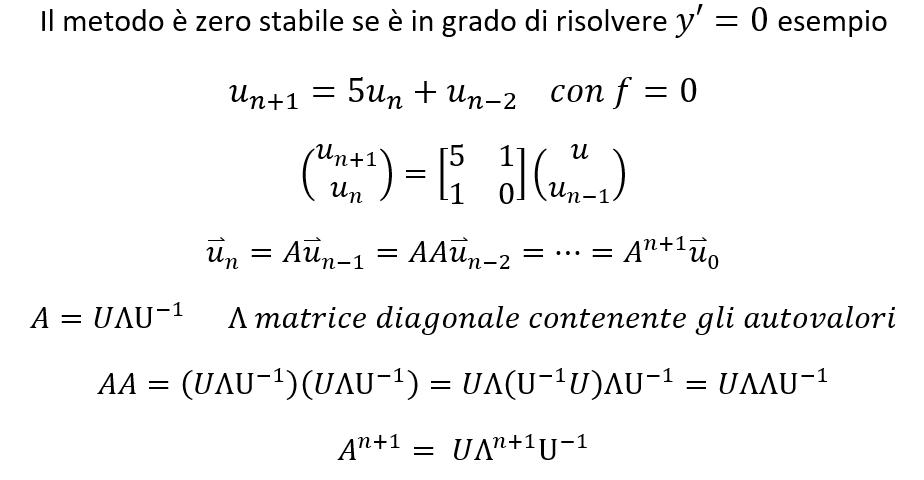
\includegraphics[width=.5\linewidth]{fig3.png}\\
       % 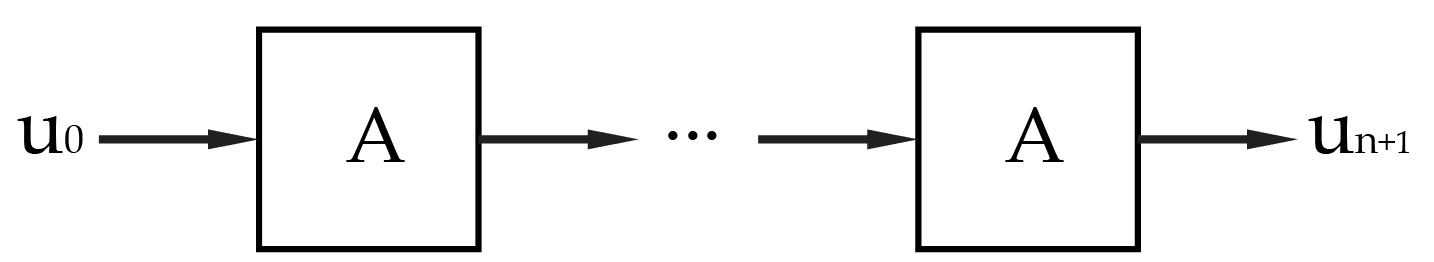
\includegraphics[width=.4\linewidth]{fig4.png}
        %\label{fig:my_label}
       % \end{figure}

       \begin{center}




\tikzset{every picture/.style={line width=0.75pt}} %set default line width to 0.75pt

\begin{tikzpicture}[x=0.75pt,y=0.75pt,yscale=-1,xscale=1]
%uncomment if require: \path (0,377); %set diagram left start at 0, and has height of 377

%Straight Lines [id:da6413889010993787]
\draw    (219.75,42.5) -- (242.75,42.5) ;
\draw [shift={(244.75,42.5)}, rotate = 180] [color={rgb, 255:red, 0; green, 0; blue, 0 }  ][line width=0.75]    (10.93,-3.29) .. controls (6.95,-1.4) and (3.31,-0.3) .. (0,0) .. controls (3.31,0.3) and (6.95,1.4) .. (10.93,3.29)   ;
%Shape: Rectangle [id:dp2986809547616538]
\draw   (249.75,27.5) -- (279.75,27.5) -- (279.75,57.5) -- (249.75,57.5) -- cycle ;
%Straight Lines [id:da425759494133338]
\draw    (284.75,42.5) -- (307.75,42.5) ;
\draw [shift={(309.75,42.5)}, rotate = 180] [color={rgb, 255:red, 0; green, 0; blue, 0 }  ][line width=0.75]    (10.93,-3.29) .. controls (6.95,-1.4) and (3.31,-0.3) .. (0,0) .. controls (3.31,0.3) and (6.95,1.4) .. (10.93,3.29)   ;
%Straight Lines [id:da27927127529816453]
\draw    (336.25,42.5) -- (359.25,42.5) ;
\draw [shift={(361.25,42.5)}, rotate = 180] [color={rgb, 255:red, 0; green, 0; blue, 0 }  ][line width=0.75]    (10.93,-3.29) .. controls (6.95,-1.4) and (3.31,-0.3) .. (0,0) .. controls (3.31,0.3) and (6.95,1.4) .. (10.93,3.29)   ;
%Straight Lines [id:da4618389576336408]
\draw    (401.25,42.5) -- (424.25,42.5) ;
\draw [shift={(426.25,42.5)}, rotate = 180] [color={rgb, 255:red, 0; green, 0; blue, 0 }  ][line width=0.75]    (10.93,-3.29) .. controls (6.95,-1.4) and (3.31,-0.3) .. (0,0) .. controls (3.31,0.3) and (6.95,1.4) .. (10.93,3.29)   ;
%Shape: Rectangle [id:dp45653346798672434]
\draw   (370,30) -- (400,30) -- (400,60) -- (370,60) -- cycle ;

% Text Node
\draw (198,39) node [anchor=north west][inner sep=0.75pt]  [font=\normalsize] [align=left] {$\displaystyle u_{0}$};
% Text Node
\draw (259.4,37) node [anchor=north west][inner sep=0.75pt]  [font=\normalsize] [align=left] {$\displaystyle A$};
% Text Node
\draw (316,43) node [anchor=north west][inner sep=0.75pt]  [font=\normalsize] [align=left] {$\displaystyle ...$};
% Text Node
\draw (429,37) node [anchor=north west][inner sep=0.75pt]  [font=\normalsize] [align=left] {$\displaystyle u_{n+1}$};
% Text Node
\draw (380.6,38.6) node [anchor=north west][inner sep=0.75pt]  [font=\normalsize] [align=left] {$\displaystyle A$};


\end{tikzpicture}

       \end{center}

\end{frame}

    \begin{frame}{Zero stabilità e convergenza (II)}
        \begin{itemize}
            \item \textbf{Se gli autovalori hanno modulo $>1$}, al passo n-esimo $A^{n+1}$ avrà coefficienti enormi. \\ Nel nostro caso, gli autovalori sono  $0.19258$ e \alert{$5.19258$}
<<<<<<< HEAD
            \item Al ventesimo passo, la $A^{n+1}$ sarà:
            %\[ 1.0e\+14 \]
            \vspace{0.5cm}
            \begin{center}
                \[\begin{bmatrix}
                1.958*10^{14} & 0.377*10^{14} \\
=======
            \item Al ventesimo passo, la $A^{n+1}$ sarà:
            %\[ 1.0e\+14 \]
            \vspace{0.5cm}
            \begin{center}
                \[\begin{bmatrix}
                1.958*10^{14} & 0.377*10^{14} \\
>>>>>>> 12a297c... aggiornate slides, rimosso submodule
                0.377*10^{14} & 0.0726*10^{14}
                \end{bmatrix} \]
            \end{center}
            \vspace{0.5cm}

            %\begin{figure}
           % \flushleft
            %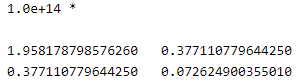
\includegraphics[width=.4\linewidth]{fig5.png}
            %\label{fig:my_label}
            %\end{figure}
<<<<<<< HEAD

=======

>>>>>>> 12a297c... aggiornate slides, rimosso submodule
            Qualsiasi perturbazione introdotta (anche nei valori iniziali) \textbf{farà divergere il metodo per qualsiasi sistema sotto analisi}.
            \medskip
            \medskip
            \item Autovalori di BDF2 (zero stabile): $1$ e $1/3$
<<<<<<< HEAD
        \end{itemize}
=======
        \end{itemize}
>>>>>>> 12a297c... aggiornate slides, rimosso submodule
    \end{frame}

    \begin{frame}{Zero stabilità e convergenza (III)}
<<<<<<< HEAD
        \textbf{Concludendo}: il metodo è \textbf{zero stabile} se tutte le radici $\xi_i$ (autovalori associati al metodo) del polinomio caratteristico $\rho(\xi)$ soddisfano $|\xi_i|\leq1$, in cui
=======
        \textbf{Concludendo}: il metodo è \textbf{zero stabile} se tutte le radici $\xi_i$ (autovalori associati al metodo) del polinomio caratteristico $\rho(\xi)$ soddisfano $|\xi_i|\leq1$, in cui
>>>>>>> 12a297c... aggiornate slides, rimosso submodule
        $$
            \rho(\xi)=\displaystyle\sum_{j=0}^k \alpha_j\xi^{k-j}
        $$
    \end{frame}

\section{Ordine e consistenza}\label{sec:sec8}
    \begin{frame}{Ordine e consistenza }
        \begin{itemize}
            \item Per i metodi LM questa operazione risulta particolarmente semplice.
        \end{itemize}
        \begin{itemize}
            \item Come visto a lezione per il caso Eulero all'indietro, analizziamo l'errore di troncamento e vediamo se è trascurabile rispetto a $h^p$.
            \item Si dice che il metodo ha ordine $p$ se l'errore di troncamento locale $d_n = O(h^p)$.
            \item Si dice che un metodo è consistente se $\rho(1) = 0$ \space e \space $\rho'(1) = \sigma(1)$ in cui:\\
            \[\rho(\xi) = \displaystyle\sum_{j=0}^k \alpha_j\xi^{k-j}\]  \space\space\space \[\sigma(\xi) = \beta_0\xi \] \\

            \item diamo un'infarinatura intuitiva sull'ordine di convergenza:
            %\item Lo stesso ragionamento viene applicato ai metodi multistep tramite opportuno operatore lineare.
            %\item Lo sviluppo di Taylor ricavato per più step sarà:
        \end{itemize}

          %\[L_{h}y(t) = C_0y(t) + C_1hy'(t) + ... + C_qh^qy^{(q)}(t) + ...   \textnormal{ in cui }\]
          %\[ C_0 = \displaystyle\sum_{j=0}^k \alpha_j \textnormal{ e }  C_i = (-1)^i \biggl[{1 \over i!}\displaystyle\sum_{j=1}^k %j^i\alpha_j  + {1 \over (i - 1)!} \beta_0\biggl] \textnormal{ con } i = 1, 2, 3, ...\]
          %\[ \textnormal{ L'errore di troncamento locale è } d_n = {L_h[y(t_n)] \over h} \textnormal{ in cui  } y(t_n) \textnormal{ è la %soluzione esatta al punto } t = t_n .\]
    \end{frame}

\begin{comment}
\begin{frame}{Ordine e consistenza (I)}
        \begin{itemize}
            \item Si dice che il metodo ha ordine $p$ se l'errore di troncamento locale è $d_n = O(h^p)$.
        \end{itemize}
        \begin{itemize}
            \item E' possibile tradurre questa informazione in $C_i$, diremo che il metodo è di ordine $p$ se:
        \end{itemize}
        \[ C_0 = C_1 = ... = C_p = 0 \textnormal{ con } C_{p+1} \not= 0 \]
         \begin{itemize}
            \item E' possibile inoltre dimostrare che il metodo è consistente se e solo se:
        \end{itemize}
        \centering$ \displaystyle\sum_{j=0}^k \alpha_j = 0  $ \space\space\space  e\space\space \space  $  \displaystyle\sum_{j=1}^k j\alpha_j + \displaystyle\sum_{j=0}^k \beta_j = 0$
        \begin{itemize}
            \item Scrivendo i polinomi caratteristici del metodo:\\
            \centering$ \rho(\xi) = \displaystyle\sum_{j=0}^k \alpha_j\xi^{k-j}$  \space\space\space \sigma(\xi) = \displaystyle\sum_{j=0}^k \beta_j\xi^{k-j} $\\
            \flushleft la condizione di consistenza diventa (se e solo se) per $\rho(1) = 0$ e $\rho'(1) = \sigma(1)$.
        \end{itemize}
   \end{frame}


\begin{frame}{Ordine e consistenza (Parte Nuova) - (I)}
          \begin{itemize}
            \item L'ordine di un metodo BDF indica con quanta precisione quest'ultimo approssima la soluzione esatta.
            \item Supponiamo di conoscere la soluzione esatta y di un sistema e di valutarla in 3 punti distinti ($ t_n, t_{n+1}, t_{n+2} $).
            Utilizzando un metodo BDF1 siamo in grado di ricostruire la soluzione con la retta che interpola i primi 2 punti.
            Scegliendo invece un metodo BDF2 ricostruiamo la soluzione con una parabola che interpola i 3 punti.
            \item Come è possibile notare dal grafico il metodo BDF2 approssima molto meglio la soluzione rispetto al metodo BDF1. Si dice quindi che BDF2 ha ordine maggiore di BDF1.
            \item Maggiore è l'ordine di un metodo migliore sarà l'approssimazione della soluzione esatta \newline \(\rightarrow\) un metodo a più step approssimerà meglio la funzione proprio per il suo \textbf{ordine} maggiore
        \end{itemize}
 \end{frame}
\end{comment}


\begin{frame}{Ordine e consistenza (II)}
        \begin{figure}
        \centering
        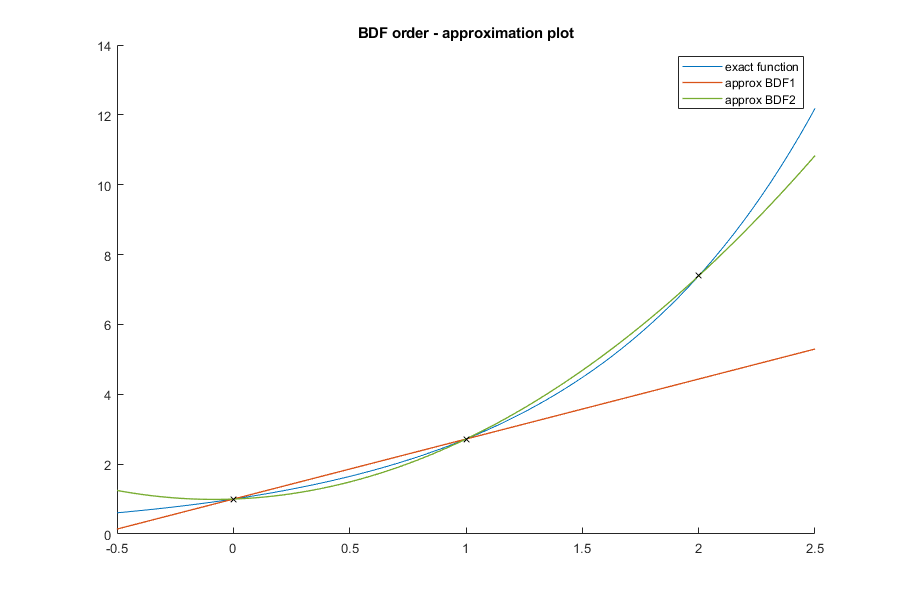
\includegraphics[width=.75\linewidth]{order.png}
        \label{fig:ordine_interpol}
        \end{figure}
 \end{frame}
 \begin{comment}

    \begin{frame}{Assoluta stabilità per metodi LM}
        Per i \textbf{multistep} si analizza la regione di NON stabilità: $z= h\lambda = {\rho(e^{j\theta})\over \sigma(e^{j\theta})}$ con $\theta \in [0,2\pi]$
        $$
            \rho(\xi)=\displaystyle\sum_{j=0}^k \alpha_j\xi^{k-j}
        $$
        $$
            \sigma(\xi)=\displaystyle\sum_{j=0}^k \beta_j\xi^{k-j}
        $$
        in cui i coefficienti $\alpha_j$ e $\beta_j$ sono tratti dalla formula che descrive i metodi:
        $$
            \displaystyle\sum_{j=0}^k \alpha_jy_{n-j}=h\displaystyle\sum_{j=0}^k \beta_jf_{n-j}
        $$
    \end{frame}
 \end{comment}
 \section{Assoluta stabilità}%\label{sec:sec10}
    \begin{frame}{Assoluta stabilità}
        \begin{figure}
        \centering
        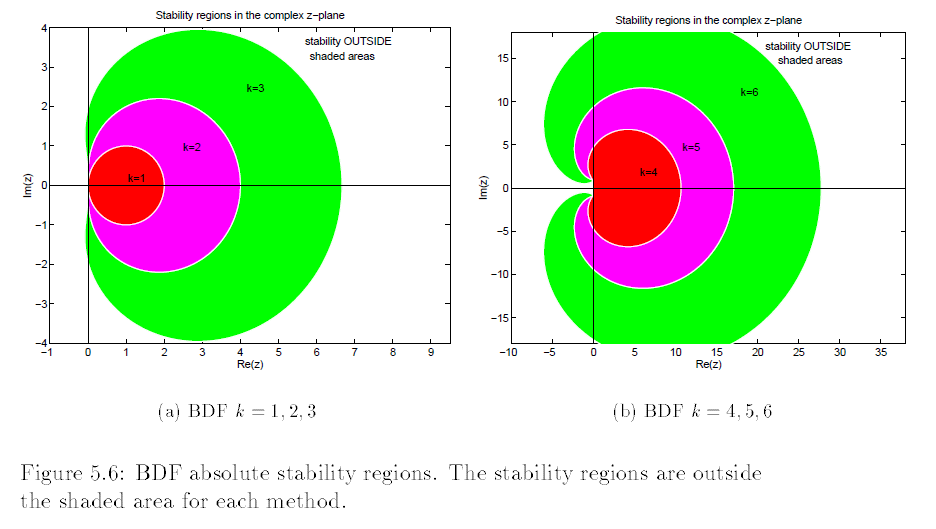
\includegraphics[width=.7\linewidth]{fig7.png}
        \label{fig:abs_stability}
        \end{figure}
        Per i \textbf{multistep} si analizza la regione di NON stabilità
        \begin{itemize}
            \item Siamo già familiari con la zona di non stabilità di BDF1
            \item Da BDF3 la risoluzione può eccitare dei modi instabili in $\operatorname{\mathbb{R}e}<0$ che faranno \textbf{divergere} la soluzione
            \item Da BDF7 si \textbf{perde la zero-stabilità}
        \end{itemize}
    \end{frame}

\section{Stiff decay}\label{sec:sec11}
\begin{comment}
    \begin{frame}{Stiff Decay}
        È una proprietà associata al metodo di risoluzione.
        Non è una buona idea accontentarsi dell’A-stabilità (stabilità nel semipiano dei reali negativi) quando si parla specialmente di sistemi stiff.
        Infatti, ci sono due casi in cui non è una condizione sufficientemente stringente:
        \begin{itemize}
            \item $\Re(\lambda)<<1$ (autovalori a velocità molto alta)
            \item $1<<\Re(\lambda)\leq0$ e $|\Im(\lambda)|>>1$ (grandi oscillazioni per valori complessi vicini all’asse immaginario
        \end{itemize}
        Considerando l’equazione di test $y'= \lambda(y-g(t))$, riscrivibile come $\epsilon y'= \epsilon\lambda(y-g(t))$ dove $\epsilon=\frac{1}{Re(\lambda)}$, si noti che per $\epsilon=0$ si ottiene la soluzione $y(t) = g(t)$. \\
        Questo si motiva dicendo che il metodo di discretizzazione ha \textit{stiff decay} se fissato $t_n>0$, $|y_n-g(t_n)|\rightarrow 0$ per $h_n\Re(\lambda)\rightarrow -\infty$.\\
        \medskip
        \medskip
        Analizzando il metodo di \textbf{Eulero all’indietro} si conclude che esso ha stiff decay, infatti applicando l’equazione $\epsilon y'= \epsilon\lambda(y-g(t))$ si ottiene: $$y_n-g(t_n)=(1-h_n-\lambda)^-^1(y_n_-_1-g(t_n))$$
    \end{frame}
\end{comment}


    \begin{frame}{Stiff Decay}
        %Questo non vale per il metodo di Eulero in avanti che non ha stiff decay.\\
        \medskip
        \medskip
        \begin{itemize}
        \item È un \alert{indice} che rivela quanto un metodo di risoluzione sia veloce nell’assestarsi alla soluzione di un sistema stiff.\\
        \item I metodi con \textit{stiff decay} \textbf{trascurano la parte della soluzione che
        varia velocemente} senza perdere dettagli nella parte a bassa velocità.
        \item I metodi BDF hanno proprietà di stiff decay
        \end{itemize}
        \begin{figure}
        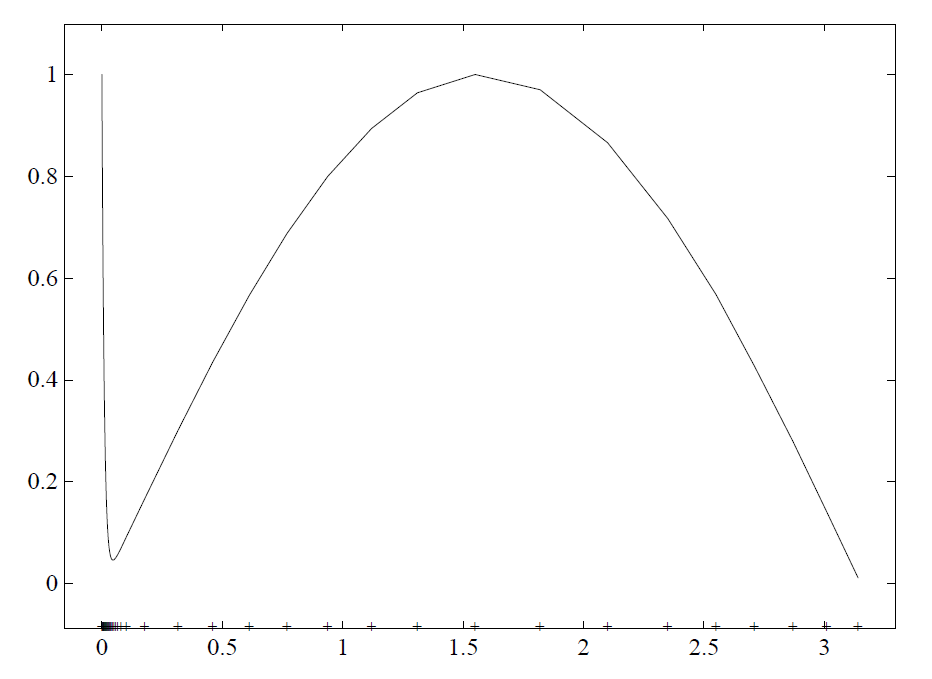
\includegraphics[width=.4\linewidth]{fig9.png}
        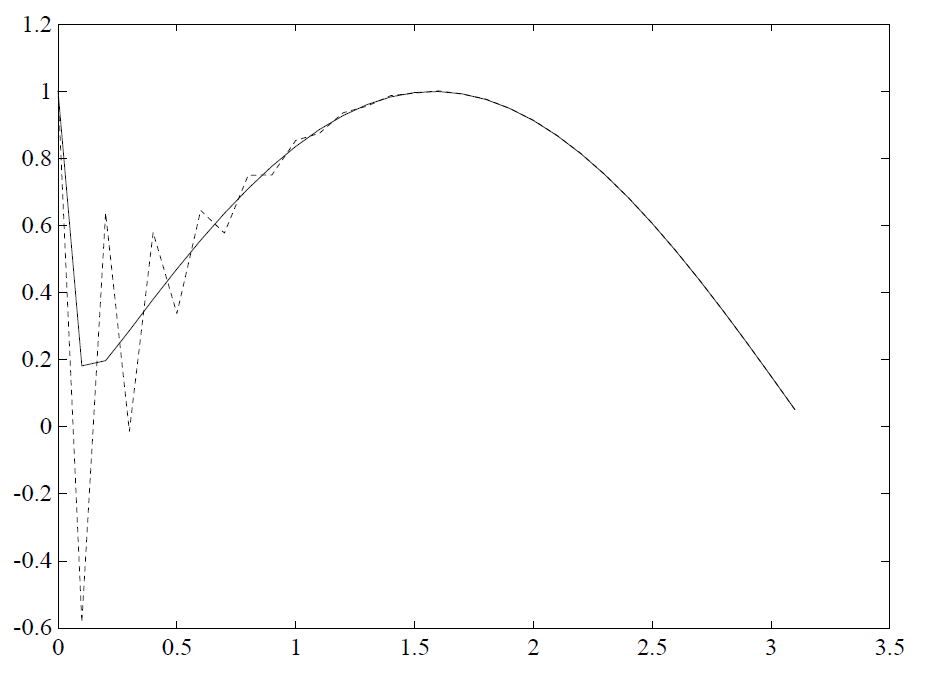
\includegraphics[width=.4\linewidth]{fig8.png}
        \label{fig:stiff_decay}
    \end{figure}
        \begin{centering}
            Linea tratteggiata $\rightarrow$ \textbf{Crank-Nicholson} \space\space\space Linea continua $\rightarrow$ \textbf{BDF1}\\
        \end{centering}
    \end{frame}

<<<<<<< HEAD
\section{Circuito RLC: soluzioni con BDF}\label{sec:sec12}
=======
\section{Circuito RLC: soluzioni con BDF}\label{sec:sec12}
>>>>>>> 12a297c... aggiornate slides, rimosso submodule

 \begin{frame}{Circuito RLC: soluzioni con BDF}
    \begin{figure}
        \centering
        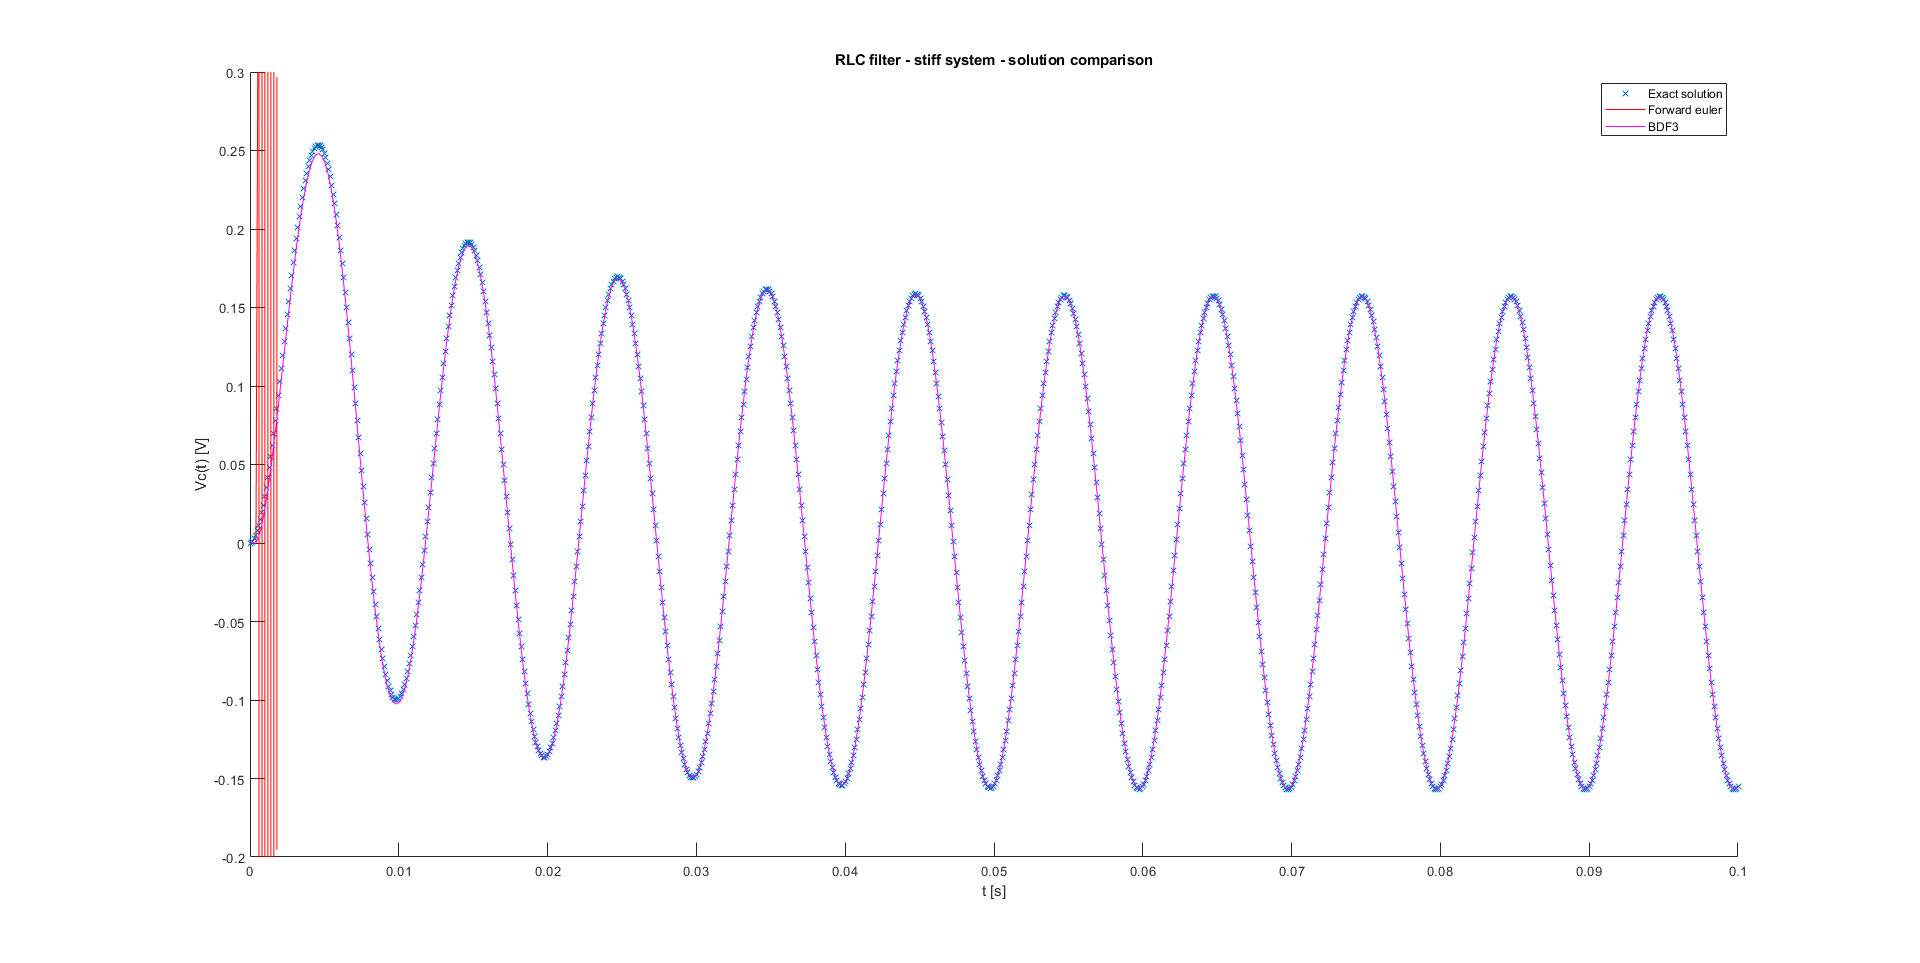
\includegraphics[width=.68\linewidth]{rlc_solution_comparison.png}
        \label{fig:rlc_bdf_solution}
    \end{figure}
<<<<<<< HEAD

=======

>>>>>>> 12a297c... aggiornate slides, rimosso submodule
    \begin{itemize}
        \item{\makebox[2.5cm]{\textbf{Eulero esplicito}\hfill} $\rightarrow 50*10^3$ passi necessari}
        \item{\makebox[2.5cm]{\textbf{BDF3}\hfill} $\rightarrow$ \space $1*10^3$ passi necessari (tempo di risoluzione $<1s$)}
    \end{itemize}
 \end{frame}
<<<<<<< HEAD


=======


>>>>>>> 12a297c... aggiornate slides, rimosso submodule
 \begin{comment}
\begin{frame}{Priming}
come risolviamo il priming in matlab
 \end{frame}


\begin{frame}{Risoluzione di equazioni non lineari con fsolve}
\begin{itemize}
    \item La funzione di Matlab \textit{fsolve} serve a risolvere sistemi di funzioni non lineari
    \item Sia \( \textbf{F}(\textbf{x}) = 0 \) una funzione vettoriale a valori vettoriali ( \( \textbf{F} : \mathbb{R}^{n*m} \rightarrow \mathbb{R}^p \) ), quindi in cui \( \textbf{x} \) può essere sia \textbf{scalare} che \textbf{matriciale}
    \item Fsolve accetta come parametri l'handler alla funzione e un valore iniziale \( x_0 \) e restituirà la corrispondente matrice \(\textbf x\)
\end{itemize}
 \end{frame}
     \begin{frame}{Circuito RLC - al variare del passo}
scegliere un metodo bdf e risolvere il circuito con diversi passi, plottando l'errore in funzione di h
 \end{frame}
 \end{comment}



\end{document}
